% TikZ-Stile und Diagramme des Berichts: Datenfluss, Zeitleiste (Architektur: architektur.tex).
% Farbkonvention: grau = bestehend, blau = in dieser Version neu, orange = Sackgasse/ersetzt.

\tikzset{
  comp/.style   = {draw=black!55, rounded corners=2pt, fill=white, align=center, font=\footnotesize, inner sep=3pt, minimum height=0.75cm},
  newc/.style   = {comp, draw=blue!70!black, fill=blue!10, line width=0.8pt},
  oldc/.style   = {comp, draw=orange!80!black, fill=orange!10, dashed},
  store/.style  = {draw=black!55, fill=white, shape=cylinder, shape border rotate=90, aspect=0.25, align=center, font=\footnotesize, minimum height=0.95cm, minimum width=1.5cm},
  newstore/.style = {store, draw=blue!70!black, fill=blue!10, line width=0.8pt},
  ext/.style    = {comp, draw=black!40, fill=black!5, dotted},
  layer/.style  = {draw=black!35, rounded corners=4pt, inner sep=7pt},
  newlayer/.style = {layer, draw=blue!60!black},
  ll/.style     = {font=\scriptsize\itshape, text=black!65},
  arr/.style    = {-{Stealth[length=2.2mm]}, black!70, line width=0.5pt},
  narr/.style   = {-{Stealth[length=2.2mm]}, blue!70!black, line width=0.8pt},
  darr/.style   = {-{Stealth[length=2.2mm]}, black!55, dashed},
  lbl/.style    = {font=\tiny, text=black!70, fill=white, inner sep=1pt},
}

% ---------------------------------------------------------------- Datenfluss je Dokument ---
\newcommand{\datenfluss}{%
\begin{tikzpicture}[x=1cm,y=1cm,every node/.style={transform shape},scale=0.9]
  \node[comp,minimum width=2.2cm] (a) at (0,0) {Crawl\\\zDocsTotal\ PDFs};
  \node[comp,minimum width=2.2cm] (b) at (3.6,0) {TF-IDF-Modell\\Score 0--1};
  \node[comp,minimum width=2.2cm] (c) at (7.4,1.4) {Score $\ge$ 0,9\\\zTfidfHigh\ (nicht geprüft)};
  \node[comp,minimum width=2.2cm] (d) at (7.4,-0.2) {Score 0,5--0,9\\LLM-Review};
  \node[comp,minimum width=2.2cm] (e) at (7.4,-1.8) {Score $<$ 0,5\\\zTfidfNegative\ verworfen};
  \node[newc,minimum width=2.4cm] (f) at (12.2,-0.2) {\zLLMConfirmed\ bestätigt\\\zLLMRejected\ verworfen};
  \node[newc,minimum width=2.4cm] (g) at (12.2,-2.2) {OCR bei Scans\\\zOCRDone\ bearbeitet};
  \node[comp,minimum width=2.2cm,draw=blue!70!black,line width=1pt] (h) at (15.8,0.6) {Endliste\\\zFinalListed};
  \draw[arr] (a) -- (b);
  \draw[arr] (b) -- (c);
  \draw[arr] (b) -- (d);
  \draw[arr] (b) -- (e);
  \draw[narr] (d) -- (f);
  \draw[narr] (e) -- node[lbl,below]{leere Textebene} (g);
  \draw[narr] (g) -- (f);
  \draw[arr] (c) -| (h);
  \draw[narr] (f) -- (h);
\end{tikzpicture}}

% ---------------------------------------------------------------- Zeitleiste ---------------
\newcommand{\zlw}{0.9}
\newcommand{\zlms}[3]{\draw[black!60] (#1*\zlw,0.55) -- (#1*\zlw,#3); \node[anchor=south,align=center,font=\scriptsize,inner sep=1pt] at (#1*\zlw,#3) {#2};}
\newcommand{\zeitleiste}{%
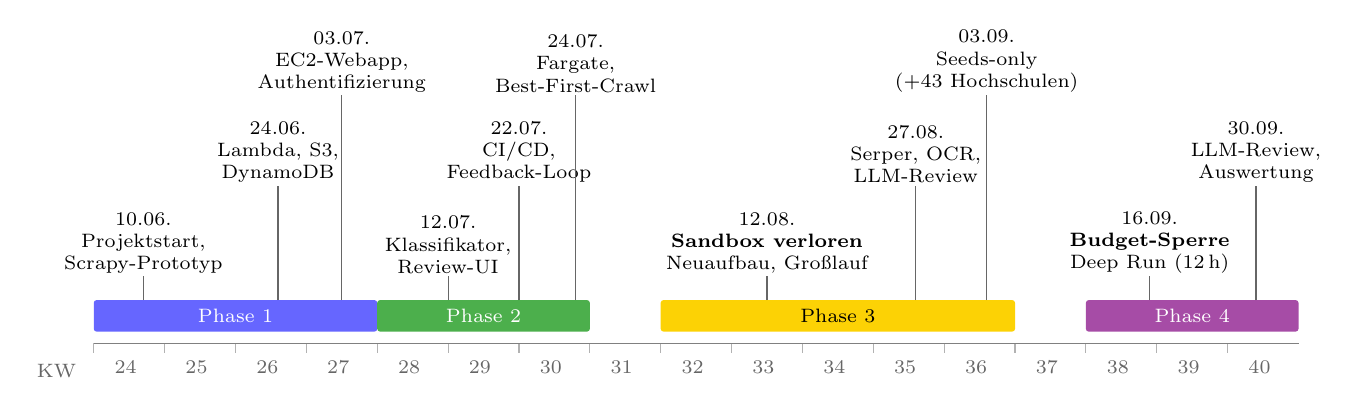
\begin{tikzpicture}[x=1cm,y=1cm,every node/.style={font=\scriptsize}]
  \foreach \k [count=\i from 0] in {24,...,40} {
    \draw[black!30] (\i*\zlw,0) -- (\i*\zlw,-0.12);
    \node[black!60,anchor=north] at (\i*\zlw+0.45*\zlw,-0.1) {\k};
  }
  \draw[black!50] (0,0) -- (17*\zlw,0);
  \node[black!60,anchor=east] at (-0.1,-0.35) {KW};
  \fill[blue!60,rounded corners=1pt] (0*\zlw,0.15) rectangle (4*\zlw,0.55);
  \fill[green!55!black!70,rounded corners=1pt] (4*\zlw,0.15) rectangle (7*\zlw,0.55);
  \fill[yellow!70!orange,rounded corners=1pt] (8*\zlw,0.15) rectangle (13*\zlw,0.55);
  \fill[violet!70,rounded corners=1pt] (14*\zlw,0.15) rectangle (17*\zlw,0.55);
  \node[white] at (2*\zlw,0.35) {Phase 1};
  \node[white] at (5.5*\zlw,0.35) {Phase 2};
  \node[black] at (10.5*\zlw,0.35) {Phase 3};
  \node[white] at (15.5*\zlw,0.35) {Phase 4};
  \zlms{0.7}{10.06.\\Projektstart,\\Scrapy-Prototyp}{0.85}
  \zlms{2.6}{24.06.\\Lambda, S3,\\DynamoDB}{2.0}
  \zlms{3.5}{03.07.\\EC2-Webapp,\\Authentifizierung}{3.15}
  \zlms{5.0}{12.07.\\Klassifikator,\\Review-UI}{0.85}
  \zlms{6.0}{22.07.\\CI/CD,\\Feedback-Loop}{2.0}
  \zlms{6.8}{24.07.\\Fargate,\\Best-First-Crawl}{3.15}
  \zlms{9.5}{12.08.\\\textbf{Sandbox verloren}\\Neuaufbau, Großlauf}{0.85}
  \zlms{11.6}{27.08.\\Serper, OCR,\\LLM-Review}{2.0}
  \zlms{12.6}{03.09.\\Seeds-only\\(+43 Hochschulen)}{3.15}
  \zlms{14.9}{16.09.\\\textbf{Budget-Sperre}\\Deep Run (12\,h)}{0.85}
  \zlms{16.4}{30.09.\\LLM-Review,\\Auswertung}{2.0}
\end{tikzpicture}}
